\documentclass{article}
% \usepackage{natbib}
\usepackage{titlesec}
\usepackage{titling}
\usepackage{geometry}
\usepackage{enumitem}
\usepackage{adjustbox}
\usepackage{chronology}
\usepackage{array}
\usepackage{booktabs}
\usepackage{listings} % Include the listings package
\usepackage{graphicx}
\usepackage{pgfgantt}
\usepackage{natbib}
\usepackage[all]{xy}
\usepackage{textcase}
\usepackage{amsmath} % Include the amsmath package for mathematical notation

\titleformat{\section}{\large\bfseries}{\thesection}{1em}{}
% Define subsection font size and formatting
\titleformat{\subsection}{\normalsize\bfseries}{\thesubsection}{1em}{}


% Define the title page layout
\geometry{a4paper, margin=1in}
\titleformat{\section}[block]{\normalfont\bfseries}{\thesection}{1em}{}
\renewcommand{\maketitlehooka}{\centering}

% Title Page Information
\title{Detecting Unsafe Updates in Software Ecosystems}
\author{Yao-Wen Chang\\Student ID: 1346258}
\date{Submission Date: September 17, 2023}
\newcommand{\supervisor}{Supervisor: Christoph Treude}
\newcommand{\industrialmentor}{Industry Mentor: Behnaz Hassanshahi (Oracle Labs, Australia)}
\newcommand{\wordcount}{Word Count:  5410 words} % Replace X with the actual word count
\renewcommand{\abstractname}{\MakeUppercase{Abstract}}


\begin{document}
\maketitle
\newpage
\tableofcontents  % This command generates the table of contents
\newpage
\begin{abstract}
The popularity of the open-source package surged, attracting more and more projects that are prone 
to deploying 3rd-party artifacts.
On the other hand, the increasing popularity of automatic CI/CD systems supports developers in 
building their projects at an extremely fast pace.
However, this convenience and the addition of new features increase the attack surface, 
providing attackers with extra ways to target downstream users

This literature review will introduce Continuous Integration/Continuous Delivery (CI/CD).
Also, potential attack surfaces and how the malicious attackers exploit these attack surfaces
to compromise CI/CD pipelines will be covered in this review. Multiple methods and 
frameworks are going to be introduced to counter the attack. 
Some method target risks at certain stage in the pipeline, and some cover the whole pipeline.

In our research, we are going to adopt the framework, Macaron, which is based on the Supply Chain Level Security Artifacts 
(SLSA) framework. We will design our method to fetch 3rd party repository from GitHub as our research data.  
\end{abstract}



\section{Introduction}
CI/CD is a development method used to efficiently build and test code updates. 
It helps organizations keep their software consistent and allows them to smoothly 
incorporate new changes. However, CI/CD systems can be tempting targets for cyber attackers. 
These attackers may try to insert malicious code into CI/CD processes, 
steal valuable credentials, or disrupt the original functioning of applications.

Recent incidence like the infection of SolarWind's Orien platform \cite{ladisa2023sok, 
peisert2021perspectives} which is used to monitor and manage the network is downloaded by 
thousands of customers, including U.S. government agencies, critical infrastrure providers, 
and private companies. 

Another malicious attack target the credentials from a contributor of the esline-scope package.
The attackers updated the malicious code within the code base, which will end up stealing
multiple credentials from the downstream users \cite{eslint2018}.

In Section 2, we delve into the related work on the CI/CD pipeline security. Three main 
attack surfaces within CI/CD pipeline and the counter measures are introduced here. 
Additionally, we will summarise the OWASP Top 10 CI/CD Risks. These will provide a comprehensive
foundation for our research. 

In Section 3, we will explore the realm of Software Supply Chain Security, which is the prerequisite
for understanding the key components of the Macaron Framework implemented in our research.
We dissect the Software Supply Chain, emphasizing the critical importance of provenance. 
Also, we will explain the nuanced difference between Software Bill of Materials (SBOM) and the SLSA Provenance.
Finally, we investigate the intricacies of the Build Model and the Security Levels specified by the SLSA framework.

In Section 4, we delineate our research aims and objectives. Our overarching aim is to fortify the security aspects of CI/CD pipelines. 
And our objectives include how we are going to achieve our aims. Furthermore, the current research 
progress and the research gap we find out in related works will be improved by our contribution.

Section 5 provides a detailed timetable and plan for the research project. 
We outline the key milestones, tasks, and deadlines necessary for successful project completion.

In Section 6, we offer a concise conclusion to the research proposal, summarizing our intentions and expectations.
\section{BACKGROUND}
A security framework provides checklist to ensure the integrity of the supply chain.
Artifacts that fulfill SLSA requirements endorsed a traceable source of the software provided
by trusted providers. SLSA provides trustworthiness of the artifacts to the developers, downstream users~\cite{slsa2023}. 

\subsection{What is Software Supply Chain?}
The software supply chain encompasses a complex network of multiple components, including both first-party and third-party libraries, 
as well as various processes integral to the development, build, testing, and publication of a software artifact. 
It serves as the backbone for delivering software products to end-users~\cite{DoDDefCI/CD2023}.

\subsection{Provenance}
SLSA provenance clearly provides the transparent information about the artifacts or the packages.
Information such as, who builds this artifact and how the artifact was built from the source.
The information will be verified by the package registry or even the customers. The provenance
is an attestation in SLSA.

\subsection{SLSA Provenance versus SBOM (Software Bill of Materials)}
Provenance and SBOM are somehow similar, so they are easily confused. Provenance is used to 
assess the trustworthiness and security of the processes used to build and deliver the software artifacts~\ref{provenance}.
By contrast, SBOM focus on listing software components and their versions \ref{SBOM}.

\begin{lstlisting}[language=, caption=SLSA Provenance, label=provenance]
[Software Build Provenance]
Build Date: 2023-09-01
Build Environment: Secure, Isolated Environment
Signing Authority: Trusted Certificate Authority (CA)
Signature Verification: Passed
[Supply Chain Processes]
Code Review: Multi-stage code review by security experts
Dependency Scanning: Automated scanning for known vulnerabilities
Build Automation: Continuous Integration/Continuous Deployment (CI/CD) pipeline
Deployment: Automated deployment to secure servers
[Organizations Involved]
Development Team: Responsible for code development
Security Team: Responsible for security reviews and scanning
Operations Team: Responsible for deployment
\end{lstlisting}

\begin{lstlisting}[language=, caption=SBOM, label=SBOM]
[MyApp (v1.0)]
Frontend Framework (v2.3)
Database Connector (v1.1)
Authentication Library (v3.0)
Logging Utility (v1.2)
\end{lstlisting}

\subsection{Build Model}
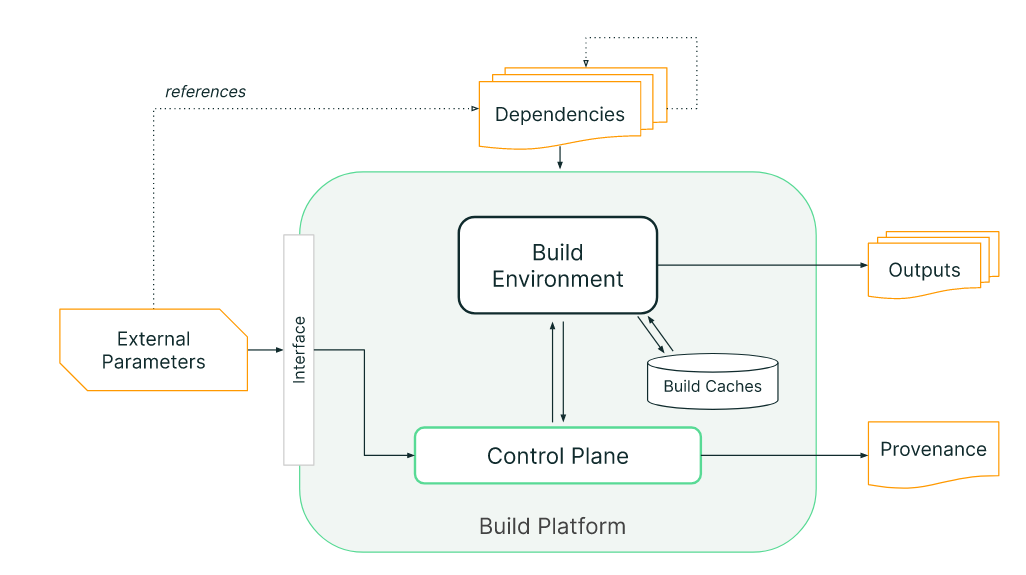
\includegraphics[width=0.7\textwidth]{./screenshot/build_model.png}
\begin{enumerate}
  \item The tenant (developers) provide specific external parameters, like the version of the application 
  and the reference to the dependency.
  \item The control plane receives the external parameters, then fetch the necessary build scripts, configuration,  
  and dependencies based on the external parameters.
  \item The control system sets up the isolated environment for the build.
  \item Finally, the model outputs the artifacts. If the build platform follows SLSA build level 2+, then
  the provenance will also be generated from the control systems.
\end{enumerate}
\subsection{SLSA Security Level}
Currently, SLSA have defined 4 levels (LV.0 - LV.3), which will be 
briefly described in Table~\ref{tab:slsa-levels}, and working on level 4.
\begin{table}[ht]
  \centering
  \caption{SLSA Security Levels}
  \label{tab:slsa-levels}
  \begin{tabular}{|c|c|p{6cm}|}
  \hline
  \textbf{Level} & \textbf{Requirements} & \textbf{Focus} \\
  \hline
  Build L0 & None & No security practices are in place. \\
  \hline
  Build L1 & With provenance & Basic security practices are followed, such as code review and basic dependency scanning. \\
  \hline
  Build L2 & Signed provenance, generated by a hosted build platform & More comprehensive security practices are implemented, including in-depth code review, vulnerability scanning, and build verification. \\
  \hline
  Build L3 & Hardened build platform & The highest level of security is maintained, with strict adherence to security practices, automated testing, and supply chain integrity checks. \\
  \hline
  \end{tabular}
\end{table}



\section{RELATED WORK}
In the beginning of the literature review, prerequisite definition of the CI/CD technique will be 
described. Then, a variety of risks and attacks are categorised based on the three attack 
surface (source code repository, build and test, and deploy) within the CI/CD pipeline.
Some defense methods introduced in the related work will be aligned with the attacks in this 
section. 
% Finally, the top ten risks existed in CI/CD pipeline referring to OWASP 2023 will be 
% summarised~\cite{OWASP2023}.

\subsection{Definition of CI/CD}
CI/CD is a development and deployment process for automatic building and testing code
changes that support organizations maintain a consistent code base, then automatically shipping 
the artifact to the target customers. 'CI' involves developers frequently merging code changes 
into a central repository where automatic builds and tests run. 'Build' is the process of 
converting source code into executable code. Then, running the automatic tests which usually 
combined unit test and integration test against unexpected results during the build process. These process will avoid integration 
challenges that can happen when waiting for release day to merge changes into the release branch. 
'CD' defined the process of the releases happened automatically~\cite{DoDDefCI/CD2023}. 

Nowadays, nearly all software applications were built on top of others works which are the third-party packages.
However, the convenience and capabilities of the third-party source code usually cause cybersecurity 
risks~\cite{mastrangelo2015use}. Software supply chain attacks aim at injecting code into software
components including source code base and artifacts, like docker image or executable software,
to compromise downstream users~\cite{ladisa2023sok, OWASP2023}. 
Some risks and counter method will be introduced in the following sections.

\subsection{Three Main Stage in CI/CD}
In the following three subsections, 
we will categorise some attack events and potential attack methods into the high-level representation 
of three main categories within the CI/CD pipeline. This categorisation allows us to gain a deeper understanding of 
the security challenges and risks associated with each phase of the software development and delivery process.
There are many strategies provided by the researchers to grapple with the tough issues presented in the software 
supply chain. 

\subsubsection{Source Code Repository}
Java Virtual Machine (JVM) executes Java bytecode and provides strong safety
guarantees. However, the unsafe API, "sun.misc.Unsafe", will cause serious 
security issue if it is misused by the developers. The research~\cite{mastrangelo2015use} 
studied a large repository, Maven, and analyzed the compiled Java code. The 
security issues include violating type safety, crashing the virtual machine (VM), 
uninitialized objects and so on. These misuse might impact third-party package 
management service. Without a manual code review from the maintainer and security inspection through automatic testing on Git repository
provider, the misused practice will not be discovered and will end up being merged in the release
artifacts. Our \textbf{Macaron} framework provide some checks to ensure the artifacts update and release
is working through a proper inspection process. The merged code should be reviewed by at least one other authenticated reviewers.
Thus, customers can trust the artifact they consume. However, the SLSA checklist does not make sure the reviewers
are capable of detecting the unsafe function call.

The research~\cite{garrett2019detecting} proposed anomaly detection method to cluster and detect 
the suspicious update JavaScript code. It shows that this unsupervised machine learning 
clustering method is able to reduce the manual review effort by 89 percent considering the worse
case that all updates are not malicious. However, the data is skewed since more unsuspicious updates
existed in the dataset. Also, the researchers choose the features based on a static method by reviewing some packages and identifying the malicious code. 
This method is less cost-efficient and only specific to the programming languages where there are models already trained. 

Nevertheless, the author in~\cite{boucher2023trojan} provide an attack approach to bypass the manual code review. 
With the Trojan source attacks, the attacker can embed seemingly unsuspicious Unicode into
the comments and indirectly modify the order of the code causing unexpected results. 
Well-designed Unicode payload would bypass the method provided by~\cite{garrett2019detecting}, 
since this feature is not recognised by the model. The author recommends the developers to include 
Regex detection method in the 'Build' stage, since this malicious code is triggered by the compiled code.
The fundamental way to avoid being compromised by the Trojan source attack is through banning the 
Unicode when it is not required in the projects. Even though recommend defense strategies 
are able to counteract this attack, but the method only deal with the specific attack against the 
CI/CD pipeline. The downstream method followed by \textbf{Macaron} is designed based on the Regex concept. Our approach
will further diagnosis the health of the code base with the automation scanning tools.

How if the update is stealthy and in the guise of the valid patch, could the manual code review by the 
professional repository maintainer and the powerful automation tools be capable of filtering out the 
malicious pull requests? Probably not. According to the research~\cite{wu2021feasibility},
there are multiple immature vulnerabilities existed in the repositories, which are usually dismissed by the maintainers, 
since they are not harmful to the software execution. However, if the remaining conditions are introduced by
the contributors intentionally or unintentionally, the performance of the artifacts will not live up to the 
maintainers' expectations. 
The author provides some effective mitigation including advanced static and dynamic analysis of the artifacts or
committer liability which is what the SLSA provenance provides. Based on quantifying the catch rate, the author is
able to understand how their attack method is possible to bypass the code review of the maintainer. In our research, 
we will also implement similar method to detect the false positive rate of our detector, the manual code review will
be conducted by ourselves.  

\subsubsection{Build/Test}
% Inject bad Dependency
% Implant CI/CD runner images and container
% Compromise CI/CD server
Malicious code injection can occur during the build of the pre-built components, especially in compiled languages.
This attack method is favored by the attackers, since the detection of the pre-built components and compiled code is 
typically more difficult~\cite{ladisa2023journey}. Opting for building package directly from 
source code is a measure to avoid this risk.

In~\cite{ohm2020backstabber}, 
an overview of the attack methods and how the attacks are triggered are being summarised. 
The most frequent way implemented to inject the bad dependencies is 'Typosquatting'. It is a simple method
to modify the packages' name with a similar one. If the consumers did not carefully check the installed 
packages, the malicious dependencies will being triggered based on the trigger point designed by the 
attackers. 
Also, this research find out the popular trigger point of the malicious dependencies is at the
installation step. At the installation step, the malicious code is usually embedded in the installation
script. When the customers install the packages, the systems are directly being compromised.  
This research paper implements the taxonomy method to deduce possible trigger points and 
the possible attacks occurring within each CI/CD stage. This method provides developers a clear 
and completed checklist to prevent the potential vulnerabilities. However, this paper does not
provide the completed counter measure against the attacks.
\textbf{SLSA} indirectly addresses 'Typosquatting' issue by providing the provenance to check the origin of
the artifacts. 

\subsubsection{Deploy}
% Bypass Review
% Use admin permission to add approver
In the extremely severe attack event~\cite{gentoo-incident-report}, 
the unknown entity gain access to the GitHub repository with the higher permission from the controlled
account of the repository maintainer. The accident causes malicious code to be committed and the
attacker even trying to remove various repositories. Some good practices are implemented
in this repository. For example, the audit logs function provided by GitHub enables the Gentoo organization
to respond quickly to prevent from the extra impact. However, the Gentoo GitHub organization does not
implement 2FA to prevent the accounts from being fully compromised. Also, it does not manage the identities
correctly. \textbf{SLSA LEVEL 4} ensure the contributors are authenticated through 2FA, and the pull requests
must be reviewed by another authenticated reviewers.

\cite{vu2021lastpymile} presents a framework to detect the discrepancies of the packages on 
between source repositories and package managers. This framework can be cooperated with other tools to improve
efficient and effective. However, the research does not consider the situation that there are no
discrepancies between the source code and the published packages, but the code have already been maliciously injected.
In the framework we deploy in this research, the provenance can ensure there are no suspicious contributors contributing
to the code base, because the detail of the artifact from building to deployment are all be recorded in the provenance.



\subsection{in-toto Framework}
in-toto is an end-to-end security framework aim to protect the software supply chain. It provides a variety
of mechanism for each steps in the CI/CD to check the integrity of the previous steps. Cryptography and hash 
function are implemented in in-toto.

\textbf{Layout} is a file format to document the actors, timestamp and actions with each step of the supply chain.
It provides the information for downstream steps to verify. This information is the cryptographic hash of action, actors and some other security
related data. Therefore, the downstream steps can verify the integrity based on the hash. This is the high level structure 
compared to Link Metadata.

\textbf{Link MetaData} is a lower level structure compared to \textbf{Layout}, which provides much detailed information about each action.

\textbf{SLSA} framework adopted in our research is based on the in-toto framework.

\subsection{Conclusion}
Despite the previously introduced methods seems to address all the security issues
existed in the code base and within the CI/CD, some of them may overemphasize one 
particular approach to address software supply chain security without considering 
compounding factors that impact risk.
Some projects aim at providing single solution that conflates multiple 
objectives~\cite{melara2022software}.
For instance, SAP's Risk Explorer is designed to cultivate a community of users 
and contributors to the taxonomy. Users can explore the taxonomy by collapsing and 
expanding nodes in an attack tree. Detailed information about attack vectors, 
references, and safeguards is presented beneath the tree. 
This tool addresses all potential risks associated with an entire CI/CD pipeline, 
as referenced in~\cite{ladisa2023journey}.

Similarly, the in-toto framework is dedicated to ensuring the integrity of the supply 
chain pipeline while harmonizing multiple objectives.

The framework employed in this research is based on Supply Chain Level Security 
Artifacts (SLSA). In the following section, we will introduce and discuss Supply Chain 
Level Security Artifacts (SLSA) in more detail.

% \subsection{OWASP Top 10 CI/CD Risks\cite{OWASP2023}}
% \begin{enumerate}[label=(\arabic*)]
%     % 1
%     \item \textbf{Insufficient Flow Control Mechanisms}
    
%     \textbf{Definition: }The attacker successfully gained unauthorised access to a critical system within the CI/CD process. 
%     However, it became apparent that the compromised system lacked adequate enforcement mechanisms to rigorously 
%     approve and review the code or artifacts provided by contributors, leaving a significant gap in the security infrastructure.

%     \textbf{Impact: }
%         \begin{itemize}
%             \item The attackers can sneakily add malicious code to a repository branch. 
%             This code can either be automatically deployed to the production system or activated manually by the attackers themselves.
%             \item Upload an artifact to the artifact repository, such as a package or container, 
%             in the guise of a legitimate artifact created by the build environment and picked 
%             up by a deployment pipeline and deployed to production.
%         \end{itemize}
    
%     \textbf{Remediation:}
%     \begin{itemize}
%         \item Configure strict branch protection rules
%         \item Limit the usage of auto-merge rules
%         \item Prevent drifts and inconsistencies between the running code in production and its 
%         CI/CD origin.
%     \end{itemize}
%     % 2
%     \item \textbf{Inadequate identity and Access Management}
    
%     \textbf{Definition: }This risks stem from the difficulties in managing the vast amount of
%     identities. The identities are identified through personal access token, e-mail, password and so on.
%         \begin{itemize}
%             \item Overly permissive identities
%             \item Stale identities - Some identities that are not active or no longer require access but have
%             not had their account deactivated.
%             \item External identities - (1) Employees registered with email from a domain not managed by 
%             the organization (2) External collaborators are outside the organization's control.
%         \end{itemize}

%     \textbf{Impact: }
%         \begin{itemize}
%             \item Overly permissive accounts leads to a state where the attacker can compromise any user
%             account on any system within the CI/CD pipeline.
%         \end{itemize}

%     \textbf{Remediation:}
%         \begin{itemize}
%             \item Consistently checked and connected the accounts of individuals with their access rights, 
%             and eliminated any unnecessary access rights that weren't needed for their current tasks.
%             \item Ensure the identities are aligned to the principle of the least privilege, and pre-defined an expiry date 
%             for the identities' permissions.
%             \item Prevent the employees from using personal email addresses.
%             \item Avoid the shared accounts. Created the dedicated accounts for each specific context.
%         \end{itemize}
%     % 3
%     \item \textbf{Dependency Chain Abuse}

%     \textbf{Definition: }
%         Dependency chain abuse refer to an attacker's ability to abuse flaws relating to how 
%         engineering workstations and build environments fetch code dependencies. The build system downloads the 
%         malicious package instead of the one intended to be pull. There are four scenarios where the developers might be tricked.
%         \begin{itemize}
%             \item Dependency confusion - Publication of malicious packages in public repositories with the same 
%             names as those private one.
%             \item Obtain the control of the account of the package maintainer in order to upload the malicious version.
%             \item Typosquatting - Publication of similar names to those popular packages.
%             \item Brandjacking - The malicious packages were consistent with the naming convention with the trusted brand.
%         \end{itemize}

%     \textbf{Impact: }
%         Once the malicious code is running, it can be leveraged for credentials theft and move horizontally through a system and 
%         network.

%     \textbf{Remediation:}
%         \begin{itemize}
%             \item Ensure the packages are not directly pulled through the internet, 
%             but through an internal proxy. And disallow pulling directly from external repositories.
%             \item Verify checksum and signature of the pulled packages.
%             \item Lock the packages' version instead of pulling the latest version.
%             \item Installation scripts should not access to 
%             sensitive resources in the build process.
%             \item Always ensure projects contain configuration files of package managers.
%             \item The most important is deployment of a quick detection, 
%             monitoring and mitigation to avoid further compromise.
%         \end{itemize}
%     % 4
%     \item \textbf{Poisoned Pipeline Execution (PPE)}

%     \textbf{Definition: }
%         The attacker access to the source control systems, but without access to the build environment, is
%         able to manipulate the build process by injecting malicious code into the build configuration file.
%         There are three type of PPE, direct PPE (D-PPE), indirect PPE (I-PPE) and public-PPE (3PE).

%         In the D-PPE scenario, the attackers modify the CI config files either by submitting a PR or directly pushing to the unprotected
%         remote branch. Since the CI pipeline execution is triggered by push or PR events, and the CI execution
%         is defined by CI Configuration file, the malicious commands run in the build node.

%         In the I-PPE scenario, the pipeline is configured to pull the CI configuration file from a protected 
%         branch or CI build is defined by the CI system instead of the in the file stored in the source code.
%         In those cases, the attackers can still inject malicious code into the files referenced by the pipeline
%         configuration file.

%         In most cases, the permissions of the access to the repository are given to the organization
%         members. However, in the 3PE scenario, the public repositories are allowed the anonymous to 
%         contribute. If the CI pipeline runs unreviewed code, the repository is susceptible to the 3PE.

%     \textbf{Impact: }
%         \begin{itemize}
%             \item Access to the secret available to the CI job.
%             \item Able to ship code and artifacts further down the pipeline, in the guise of legitimate 
%             code build by the build process.
%         \end{itemize}

%     \textbf{Remediation:}
%         \begin{itemize}
%             \item Ensure that pipelines running unreviewed code are executed on isolated nodes to prevent
%             exposure of sensitive information.
%             \item To prevent the manipulation of the CI configuration file.
%             \item Remove permissions from the users that do not need them.
%         \end{itemize}
%     % 5
%     \item \textbf{Insufficient PBAC (Pipeline-Based Access Controls)}

%     \textbf{Definition: }
%         Adversary is able to execute malicious code within the context of the pipeline.
%         The pipeline execution nodes have access to the resources or systems within and outside the 
%         execution environment.

%     \textbf{Impact: }
%         Malicious code is able to run in the context of the pipeline. Probability, this attack would lead to 
%         the exposure of the secret and confidential data.
        
%     \textbf{Remediation:}
%         \begin{itemize}
%             \item Do not use shared node for pipeline with different levels of sensitivity.
%             \item Where applicable, run pipeline jobs on a separate, dedicated node.
%         \end{itemize}
%     % 6
%     \item \textbf{Insufficient Credential Hygiene}

%     \textbf{Definition: }
%         CI/CD environments are built of multiple systems communicating and authenticating against each other
%         through verifying the credentials. Insufficient credential Hygiene generally means the overly permissive
%         or the credentials are accidentally existed in CI/CD pipelines and the code repositories. Some cases are
%         due to the unrotated credentials issue.  

%     \textbf{Impact: }
%         The adversary obtains the credentials to deploy the malicious code and artifacts.
%     \textbf{Remediation:}
%         \begin{itemize}
%             \item Conform to the least privilege rule and granted the exact set of permission.
%             \item Avoid sharing the same sets of credentials across multiple contexts.
%             \item Using temporary credentials. If using static credentials, better periodically rotate
%             all the static credentials and detect stale credentials.
%             \item Scoping the credentials to specific source IP to ensure the credentials cannot be used
%             outside the environment even if it is compromised.
%             \item Detect secrets pushed to the code repositories.
%         \end{itemize}
%     % 7
%     \item \textbf{Insecure System Configuration}

%     \textbf{Definition: }
%         Flaws in the security settings and configuration, which often results in easily compromised by The
%         attackers. For example, the overly permissive network access controls allow the attackers to interact
%         with different domain.

%     \textbf{Impact: }
%         The flaws may be abused by the attacker to manipulate CI/CD flows, and obtain the sensitive tokens.
    
%     \textbf{Remediation:}
%         \begin{itemize}
%             \item Ensure the network access the systems is aligned with the principle of the least access.
%             \item Periodically review all system configuration.
%             \item Ensure permission to pipeline execution nodes follow the least privilege principle. 
%         \end{itemize}
%     % 8
%     \item \textbf{Ungoverned Usage of 3rd Party Services}

%     \textbf{Definition: }   
%         3rd party services are granted access to the organization's assets, such as the CI/CD systems.

%     \textbf{Impact: }
%         Lack of governance and visibility around 3rd part might allow the write permission on the repository.
%         Then, the flaw is leveraged by the adversary to push the code to the repository.
%     \textbf{Remediation:}
%         \begin{itemize}
%             \item Define the scoped context that the 3rd parties are able to access, and with strict ingress
%             and egress filter.
%             \item Established vetting procedures to verify the trustworthiness of the 3rd parties. Prior to being 
%             granted access to the environment, the approval of being granted to resources should be verified.
%         \end{itemize}
%     % 9
%     \item \textbf{Improper Artifact Integrity Validation}

%     \textbf{Definition: }
%         This flaw allows an attacker with access to the CI/CD process to push malicious code or artifacts down 
%         the pipeline.

%     \textbf{Impact: }
%         Execution of malicious code.

%     \textbf{Remediation:}
%         \begin{itemize}
%             \item Validate the integrity of resources all the way from development to production.
%             \item Code signing to prevent unsigned commits from flowing down the pipeline.
%             \item Prior to fetching and using 3rd parties, the hash of the 3rd parties should be calculated and 
%             cross-referenced against the official published hash of the resource provider.
%         \end{itemize}
        
%     % 10
%     \item \textbf{Insufficient logging and visibility}

%     \textbf{Definition: }
%         The risk allow the adversary to carry out malicious activities without being detected.
%         For example, the permission modification and execution of builds.

%     \textbf{Impact: }
%         Fail to detect a breach may face difficulties in mitigation. Time and data are the most 
%         valuable commodities to an organization under the attack.

%     \textbf{Remediation:}
%         \begin{itemize}
%             \item First, be familiar with different systems involved in the potential threats.
%             \item Make sure all relevant logs are enables.
%             \item Shipping logs to a centralized location and creating the alerts to detect malicious activities.
%         \end{itemize}
% \end{enumerate}

% \subsection{How SLSA Framework Solve Frequent Risks in CI/CD}
% In this section, we will provide some examples to show how SLSA is able to mitigate the risks listed in OWASP Top10.
% SLSA specifies a list of requirements which will enforce secure practice against the most frequent risks.
% In the \textbf{Two-person Reviewed}, it requires the pull request being reviewed by another authentic reviewer.
% The method will make \textbf{Insufficient Flow Control Mechanisms} risk impossible.
% Also, \textbf{Dependencies Complete} is to make sure the SLSA provenance records all dependencies during
% build step. Then, the developers can trust the provenance and inspect all dependencies. This requirement 
% will indirectly defense \textbf{Dependency Chain Abuse}.



% \subsection{ U.S. Department of Defense Recommend \cite{DoDDefCI/CD2023}}
% \begin{enumerate}
%     \item \textbf{Zero Trust Approach}
    
%         No user, endpoint device or process is fully trusted.

%     \item \textbf{Strong Cryptographic Algorithm}
    
%         Avoid using outdated cryptographic algorithm which poses a threat to CI/CD pipelines.
%         The threat includes sensitive data exposure and keys generated across the CI/CD 
%         pipeline.

%     \item \textbf{Minimize the Use of Long-Term Credentials}

%     \item \textbf{Add Signature to CI/CD Configuration and Certify It}

%         Ensure the code change is continuously signed, and the signature is verified throughout
%         CI/CD process. If the signing identity itself is compromised, it undermines trust.
    
%     \item \textbf{Two-Person Rules for all Code Updates}

%         The developer checks in the code which should be reviewed and approved by another 
%         developer. 

% \end{enumerate}



\section{METHODOLOGY}
According to previous works from other researchers, most of the works mainly focus on detecting the malicious
code within the source code base. Despite this traditional method might be able to discover the suspicious 
code through scanning, it is an inefficient process if the code base is frequently updated. Also, the method 
can only promise the malicious code within the whitelist to be detected. However, the attackers usually 
figure out possible payloads or injection methods to bypass the automatic scanning, like the Trojan source 
attacks~\cite{boucher2023trojan} we introduced before. 
Some works recommend to use machine learning method to detect malicious code as an outlier~\cite{garrett2019detecting}.
How if the attacker try to bypass the training model with obfuscation method? Finding out proper features for
training a model is time-consuming. The research ~\cite{zheng2023careful} discover a method to modify
the forward function in deep learning model, which will indirectly poison the downstream developers who build 
their model based on the incorrect pretrained weight. 
Therefore, we are thinking of whether developing a method to grapple with malicious code injection is possible.
If our framework can make sure the contributors are not being compromised and the CI/CD configuration follows
the safe requirements suggested by security experts, the developers can trust the dependencies that are
used in their project. 
In order to efficiently check the safety of the artifacts, our research will focus on contributing to the Macaron
Framework which is based on SLSA requirements.

Three major questions will be addressed in this research:
\begin{enumerate}
    \item[{\textbf{RQ1:}}] What are the top five frequently emerging risks that exist within popular Python and Java repositories?
    \item[{\textbf{RQ2:}}] What is the intent behind these suspicious updates from contributors in open source projects?
    \item[{\textbf{RQ3:}}] How can maintainers enhance the security of their CI/CD pipelines based on the findings and recommendations from our research?
\end{enumerate}

\begin{center}
    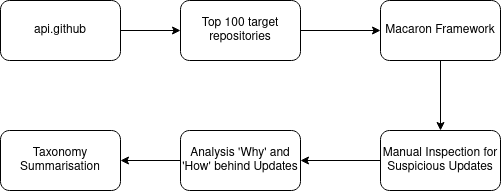
\includegraphics[width=0.7\textwidth]{./screenshot/research_flow.png}
\end{center}

\subsection{Research Aims}
This research is aim to contribute the Macaron framework, then examine top 100 Python and Java Git 
repositories with this framework. The statistical findings will be further concluded through the further process.
Also, the results will provide the developers and maintainers with a good understanding 
of the vulnerabilities existed in their CI/CD pipelines configuration. Furthermore, the reason behind
these unsafe update will be deeply investigated.

\subsection{Research Objectives}
\begin{enumerate}
    \item First step: Fetch the repositories build from Python and Java with the top 100 most stars.
    \item Second step: Input the repositories name into the Macaron Framework to analysis. 
    \item Third step: Summarize the outputs generated by Macaron and visualize the results with graphs.
    \item Fourth step: Manually inspecting the code base from the potentially problematic repositories 
    due to not comply with the requirements from the SLSA.
    \item Fifth step: Document and investigate the reason for this suspicious updates.  
\end{enumerate}

\section{Timetable / Plan}
We split the research plan into three phases, also, providing a timetable for understanding 
the research schedule.

\subsection{Phase One}
Defining Unsafe Updates: Building on similar research conducted in the JavaScript ecosystem 
\\(https://ieeexplore.ieee.org/document/8805698), the project's first phase 
involves defining what an unsafe update means within the context of Python and/or Java. 
Typically, an unsafe update could be one that introduces breaking changes, 
negatively affects performance, opens up security vulnerabilities, 
or adds incompatible API changes.

In order to discover different type of unsafe updates and the target victim, we will review 
related work, articles, and CI/CD attack events to support the understanding of the CI/CD 
attacks existed nowadays. 

\subsection{Phase Two}
Implementation of Safety Checks: Next, we will extend the Macaron framework's 
functionality by implementing additional safety checks for these unsafe updates.
Macaron is an extensible checker framework for supply chain security and CI/CD services,
such as GitHub Actions. It allows adding new checks as Python modules and provides 
intermediate representations specifically designed for CI/CD services to facilitate 
verifying new properties. We will begin from implementing SLSA Level 4 check including Two 
Person Review, Verified History, and Retained indefinitely.

The Two Person Review check ensures each pull request is reviewed by at least one authentic reviewer.
This check deal with the situation that someone wants to bypass the review and directly merge 
their code into the branch. Our method will fetch all the pull requests from the branch 
specified by the users of Macaron Framework.

The Verified History ensures at least one strong authenticated participant of the revision's history.
The identities should be authenticated through two-step verification. The first step usually 
verified the password, and second step might be verified through SMS or Email. This check grapple
with the situation when the identities' account are being compromised.

Retained indefinitely will check if the commits are preserved for 18 months; therefore, the
consumers can trust the artifacts they are going to use in their applications are not being 
modified by suspicious contributors.

The remaining session, we will keep contributing to the framework, but only implementing a
specific version on the phase three.
\subsection{Phase Three}
Empirical Analysis of Real-World Projects: With the safety checks in place, 
the final phase of the project is an empirical study conducted on GitHub to ascertain
the frequency of unsafe updates occurring in Python and/or Java projects.
By understanding the 'how' and 'why' behind these updates, developers can adopt more 
informed, proactive strategies in their coding practices.

Furthermore, we will build graph and even attack tree to classify our finding and visualize 
the result. In this way, the developers can easily understand what they should focus 
and improve in their current configuration of the CI/CD pipeline or the future projects.


\newganttchartelement{orangebar}{
    orangebar/.style={
        inner sep=0pt,
        draw=red!66!black,
        very thick,
        top color=white,
        bottom color=orange!80
    },
    orangebar label font=\slshape,
    orangebar left shift=.1,
    orangebar right shift=-.1
}

\newganttchartelement{bluebar}{
    bluebar/.style={
        inner sep=0pt,
        draw=purple!44!black,
        very thick,
        top color=white,
        bottom color=blue!80
    },
    bluebar label font=\slshape,
    bluebar left shift=.1,
    bluebar right shift=-.1
}

\newganttchartelement{greenbar}{
    greenbar/.style={
        inner sep=0pt,
        draw=green!50!black,
        very thick,
        top color=white,
        bottom color=green!80
    },
    greenbar label font=\slshape,
    greenbar left shift=.1,
    greenbar right shift=-.1
}

\begin{center}
\resizebox{\textwidth}{!}{ % Resize the chart to fit the page width
\begin{ganttchart}[
  hgrid style/.style={black, dotted},
  vgrid={*5{black,dotted}},
  x unit=9mm,
  y unit chart=9mm,
  y unit title=12mm,
  time slot format=isodate,
  time slot unit=month, 
  % group incomplete/.append style={fill=groupblue},
  group label font=\bfseries \Large,
  % group progress label font=\bfseries\small,
  bar progress label node/.append style={right=7pt},
  group progress label node/.append style={right=7pt},
]{2023-7-24}{2024-5-31}
\gantttitlecalendar{year, month} \\ 
\ganttgroup[
  group/.append style={fill=orange}
]{Phase One}{2023-7-31}{2023-8-29}\\
\ganttorangebar{Literature Review}{2023-7-31}{2023-8-29}\\
\ganttorangebar{Define Unsafe Updates}{2023-7-31}{2023-8-29}\\
\ganttgroup[
  group/.append style={fill=blue}
]{Phase Two}{2023-7-31}{2024-5-31}\\
\ganttbluebar[bar height=0.5]{Implement Two Person Review Check}{2023-7-31}{2023-9-12}\\
\ganttbluebar[bar height=0.5]{Implement Verified History Check}{2023-8-27}{2023-9-30}\\
\ganttbluebar[bar height=0.5]{Implement Retained indefinitely}{2023-9-27}{2023-10-12}\\
\ganttbluebar[bar height=0.5]{Implement Other Functions}{2023-10-12}{2024-5-31}\\

\ganttgroup[
  group/.append style={fill=green}
]{Phase Three}{2023-9-18}{2024-5-31}\\
\ganttgreenbar{Collect Data}{2023-9-18}{2024-1-23}\\
\ganttgreenbar{Empirical Analysis of Real-World Projects}{2024-1-23}{2024-5-31}\\
\end{ganttchart}
}
\end{center}
\section{Conclusion and Expected Outcomes}
\subsection{Conclusion}

\subsection{Expected Outcomes}
The expected outcomes of this research will be contributing some checks properly to the Macaron 
Framework. Also, finding out vulnerabilities within the popular repositories. Our work expects to 
find out if the CI/CD pipeline configuration or the protection mechanism is strong enough to 
avoid unexpected attacks. Taxonomy technique mentioned in~\cite{ohm2020backstabber} will be 
implemented in our research to classify the discovered vulnerabilities, and finding out the potential
main goal of the attack according to these vulnerabilities. Finally, our research will expect to 
discover the reason behind these malicious updates.   

\bibliographystyle{plain} % Choose a bibliography style
\bibliography{references} % Specify your .bib file
\end{document}